\documentclass[a4paper,12pt]{report}

\usepackage[utf8]{inputenc} % damit auch äöüß gehen
\usepackage[T1]{fontenc}	% so kann man bessere wörtliche rede machen
\usepackage[ngerman]{babel} % deutsche Silbentrennung
\usepackage{gensymb} % für besondere Symbole wie zB Grad -> \degree
\usepackage{csvsimple} % for tables
\usepackage{graphicx}
\usepackage{amsmath}
\usepackage{enumitem} % um aufzählungen zu machen
\usepackage[
	colorlinks,
	pdfpagelabels,
	bookmarksopen = true,
	bookmarksnumbered = true,
	linkcolor = black,
	plainpages = false,
	hypertexnames = false,
	citecolor = black
]{hyperref} % verlinkt referenzen für die digitale verwendung

%\renewcommand{\familydefault}{\sfdefault} % NOTE: Hermann liest am Bildschirm lieber serifenlos --hoe

\usepackage{tikz}
\usetikzlibrary{datavisualization}
\usetikzlibrary{datavisualization.formats.functions}

%TODO: Einführung, Gruppenfoto (mit Auto), Passiver Schreibstil, Bilder, Allgemeine Beschreibungen der Kapitel, Autor der jeweiligen Funktion, Fazit, Zwischenfazit für jedes Kaptiel?, Sinnabschnitte,  Literatur/Quellverzeichnis

\begin{document}
	
%%%%%%%%%%%%%%%%%%%%% HEADER %%%%%%%%%%%%%%%%%%%%%

	\title{Robotik Praktikum -- Gruppe 2}
	\author{Frauke Jörgens (minf101207) \and Franz Wernicke (ite101729) \and Thorger Dittmann (ite101646) \and Jan Ottmüller (tinf101737) \and Felix Maaß (ite101754)}
	\date{\today}
	\maketitle
	
	\tableofcontents
	

%%%%%%%%%%%%%%%%%%%%%%%%%%%%%%%%%%%%%%%%%%%%%%%%%%	
\chapter{Allgemeine Themen}
\section{Lineare Funktion}

% TODO: Diese Sektion muss irgendwo einsortiert werden oder braucht eine eigene Einleitung "es gibt im system viele messwerte, die als einfache Fließkommazahlen…" --hoe

	Für manche Werte war es nötig eine Modulation hinzufügen zu können.
	
	Es wurde sich aus Gründen der besseren Visualisierung für einen eigenen ADTF Filter entschieden.
	Dieser nimmt ein Eingangssignal entgegen, welches daraufhin mit einem Gain und Offset versehen wird und anschließend den modulierten Wert zurückliefert.
	
	Diese Funktionalität entspricht einer "Linearen Funktion":
	
	\[y = g \cdot x + o\]
	
	wobei $x$ der Eingang, $g$ der Gain, $o$ der Offset und $y$ der Ausgang ist.
	\\
	Gain und Offset können hierbei sowohl über eigene Eingangspins als auch über variable Filterparameter gesetzt werden.
	

\section{Float Wert Generator}

	Um verschiedene Filter zu testen, die einen Wert als Eingang benötigen, wurde dieser Block erstellt.

	Da neue Ausgaben nur durch die Methode \texttt{OnPinEvent} ausgelöst werden, wurde ein \texttt{WatchDog} als Input definiert. So wird mit jedem Auslösen des WatchDog der Wert gesendet. Der Wert kann in den Einstellungen des Filters während der Laufzeit gesetzt werden.


\subsection{In Entwicklung}

	Es ist geplant, dass die Geschwindigkeit des Autos mithilfe des aktuellen Lenkwinkels in Kurven angepasst werden kann.

%%%%%%%%%%%%%%%%%%%%%%%%%%%%%%%%%%%%%%%%%%%%%%%%%%
\chapter{Lenkung}

%TODO: Hier ein bisschen was über die beiden Filter schreiben + Ackermann Steering Approximation + Theoretische Überlegungen auf zettel und papier
%https://en.wikipedia.org/wiki/Steering

	Standardmäßig erwartet der vorgefertigte Arduino-Controller-Filter in ADTF einen Wert zwischen $-100$ und $+100$, um den Servomotor für die Lenkung richtig zu instruieren.
	
	Es wurde eine Modularisierung eingeführt, die das Vorhaben der Ansteuerung in die im folgenden beschriebenen Bereiche aufteilt.
	
\section{Mittels Winkel}
\label{Steering-Angle-To-Servo}

	Die erste Abstraktionsebene stellt das Mapping von Lenkwinkel zu Servostellung dar.
	Hierfür ist es nötig zu wissen, welchen Wert der physikalisch bedingte maximale Lenkwinkel hat.
	
	Wir stellten fest, dass die Auslenkung der Vorderräder unterschiedlich stark erfolgt.
	Dies liegt daran, dass die Räder unterschiedlichen Radien folgen müssen, um einen gemeinsamen Kurvenmittelpunkt zu besitzen.
	Gibt es keinen Gemeinsamen, so entsteht mehr Abrieb bzw. Schlupf, was wiederum zu ungenauen Lenk- und Wegverhalten führt.
	
	Oft verwendet wird die sogenannte Ackermann-Lenkung, die genau diesem Prozess entgegenwirken soll, indem die Räder unterschiedlich stark einlenken.
	
	\paragraph{Theorie.}
	Es wurde sich für eine Annäherung der Winkel entschieden, da wir die Räder nicht getrennt anstellen können.
	Wir denken uns idealisiert ein Rad in der Mitte der Vorderachse und führen unsere Berechnungen anhand dessen durch.
	
	\begin{figure}[ht]
		\centering
		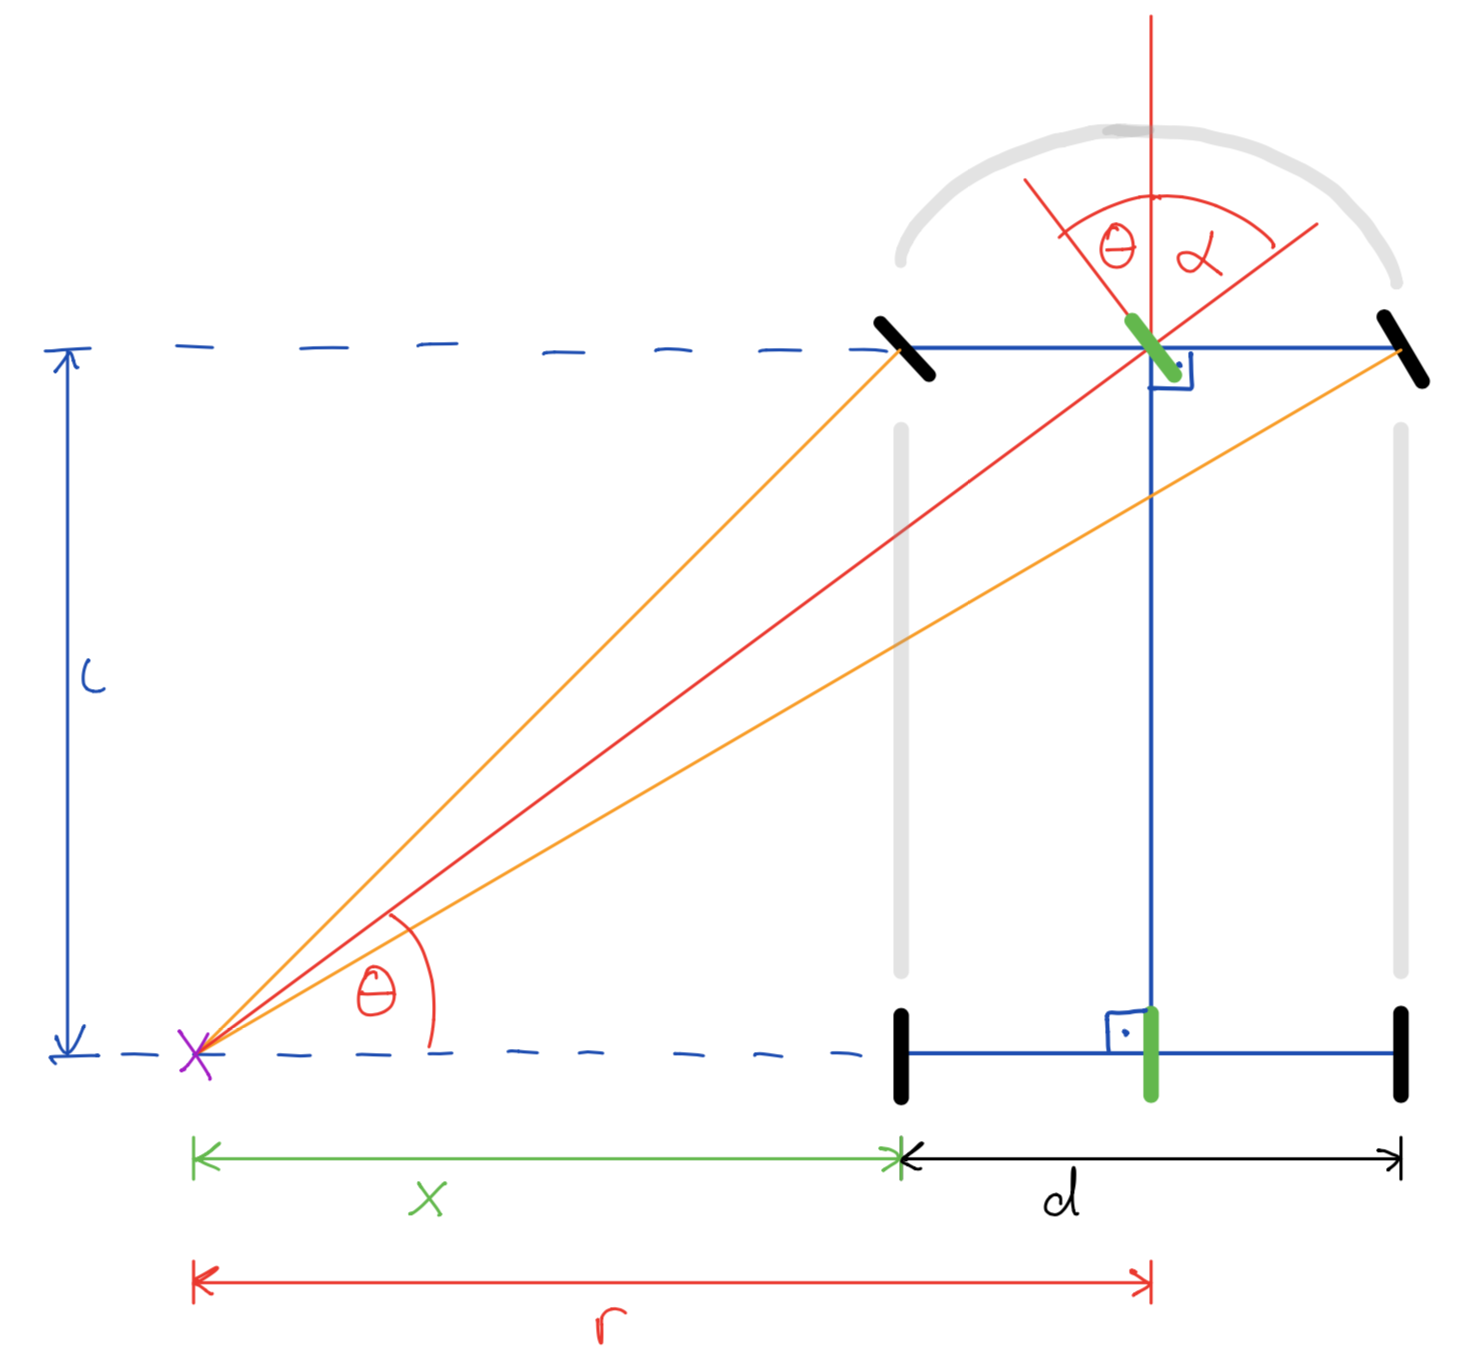
\includegraphics[width=\textwidth,height=\textheight,keepaspectratio]{assets/Lenkwinkel-Skizze.png}
		% NOTE: Skizze ist gut. --hoe
		\caption{Skizze des idealisierten Lenkwinkels}
		\label{img-steering-angles-sketch}
	\end{figure}
	\pagebreak
	
	Basierend auf den in \autoref{img-steering-angles-sketch} skizzierten trigonometrischen Überlegungen wurde folgende Gleichung entwickelt:
	
	\begin{align*}
		&&\theta_{max} &= \arctan\left( \frac{l}{r} \right)\\
		&&&= \arctan\left( \frac{l}{x_{min} + \frac{d}{2}} \right) &&\|\quad d = 260mm, l = 360mm
	\end{align*}
	\\
	Hierbei stellt $d$ die Spurweite und $l$ den Radstand dar.
	
	Aufgrund des Schlupfes erwiesen sich theoretische Werte für den minimalen Innenradius $x_{min}$ nicht als akkurat, weshalb dieser sodann durch  Praxistests % NOTE: Falls noch vorhanden, Rohdaten gerne als Anhang beilegen (eingescannter Zettel reicht mir schon) --hoe
	empirisch ermittelt wurde:
		\[x_{min} = 400mm.\] 
	
	\paragraph{Resultat.}
	Dieses Vorgehen generierte eine zufriedenstellende Lösung.
	Der maximale Lenkwinkel wurde zu $\theta_{max} \simeq 34,19\degree$ bestimmt.
	
	Es erfolgt eine Übersetzung des gewünschten Lenkwinkels von $-\theta_{max}$ bis $+\theta_{max}$ auf die nötigen Servoansteuerungswerte zwischen $-100$ und $100$.

\section{Mittels Radius}

	Die zweite Abstraktionsebene stellt den Übergang von von Kurvenradius zu Lenkwinkel dar.
	Einige notwendige Vorkenntnisse sind bereits in \autoref{Steering-Angle-To-Servo} erläutert worden.
	Darauf setzt dieser Filter nun wie folgt auf:
	
		\begin{align*}
		&&\theta\left(r\right) &= \arctan\left( \frac{l}{r} \right)\\
		&&&= \arctan\left( \frac{l}{r - \frac{d}{2}} \right) &&\|\quad d = 260mm, l = 360mm
		\end{align*}
	
	Analog zu \autoref{Steering-Angle-To-Servo} stellt $d$ die Spurweite und $l$ den Radstand dar.

	\paragraph{Resultat.}
	Soll nun ein bestimmter Kurvenradius eingestellt werden, wird der dazugehörige Winkel berechnet und daraufhin zum Servowert umgerechnet.

% TODO: Bemerken, dass sowas in ADTF schon drin ist und begründen, warum deren Filter nicht verwendet wurde. --hoe

%%%%%%%%%%%%%%%%%%%%%%%%%%%%%%%%%%%%%%%%%%%%%%%%%%
\chapter{Motorregelung}	

%%%%%%%%%%%%%%%%%%%%%%%%%%%%%%%%%%%%%%%%%%%%%%%%%%
\chapter{Kollisionsvermeidung}

	Mithilfe % TODO: Ändern in "Mit Hilfe". "Mithilfe" bedeutet "Unterstützung". --hoe
	der Ultraschallsensoren sind vorn und hinten Hindernisse zu erkennen.
	Dadurch soll es möglich sein, zu reagieren bevor eine Kollision stattfindet.

\section{Genauigkeit der Ultraschallsensoren}

	\paragraph{Situation.}
	Die Ultraschallsensoren liefern einzeln betrachtet recht akkurate Werte.
	Die Genauigkeit wurde zu $\pm1cm$ bestimmt.
	
	\paragraph{Problem.}
	Leider ist es jedoch der Fall, dass die Messungen Ausreißer aufweisen.
	Teils wurden leicht erkennbare Fehler zurückgegeben ($-1$). Teils wichen die Werte aber auch um erhebliche Beträge ab.
	
	Den Grund für Letzteres diagnostizierten wir in der gleichzeitigen Ansteuerung der Sensoren.
	Da jedoch der Code der Arduinos (welche sich um die Erfassung der Werte kümmern) nicht offen liegt, können wir vorerst keine Änderungen daran vornehmen.
	
	Damit diese falschen Werte dennoch nicht mit in kommende Berechnungen einbezogen werden, musste eine entsprechende Lösung gefunden werden.

	\paragraph{Resultat.} % TODO: Das ist nicht das Resultat, sondern die Maßnahme. In Resultat wird die Effektivität der Maßnahme (die Verbesserung durch den Filter) dargestellt. --hoe
	Zur Stabilisierung der Messwerte entschieden wir uns für eine Filterung.
	Es wurde nach einem Filter gesucht, der robust gegenüber Ausreißern ist.
	Hier kam uns als Erstes der Median in den Sinn.
	
	Ein entsprechender Filter wurde nun sowohl als C++ Klasse als auch als ADTF Filter erstellt.

	Der ADTF Filter besitzt einen Parameter, der die Fenstergröße einstellt (i.e. die Anzahl an Werten über die der Median gebildet werden soll) und ermöglicht damit eine flexible Filterung der Messwerte.

\section{Hinderniserkennung}
	
	Mit Hilfe % TODO: siehe oben --hoe
	der aufbereiteten Ultraschallsensordaten wird es möglich sein, das Auto sicher durch die Umgebung zu navigieren.
	\footnote{Dieses Feature befindet sich noch in Entwicklung.} % TODO: Whitespace vor Fußnoten entfernen. --hoe
	
\subsection{Theoretische Überlegungen}
	
	Um sich ein geeignetes Bild der Umgebung zu machen, ist es sinnvoll, jeden  Messwert der fünf Frontsensoren einzeln zu bewerten, da sonst unnötige Manöver ausgeführt werden, um Objekten auszuweichen, die nicht auf unserer Trajektorie liegen.
	Uns erschien es sinnig, dies anhand des aktuellen Lenkwinkels zu tun.
	
	Es wurde eine Funktion synthetisiert, die die Relevanz der einzelnen Messwerte zu dem Lenkwinkel in Relation setzt:
	
		\[y=2-e^{-3 \cdot \left( x-a \right)^2}\]
	
	Sie bietet eine Gewichtung für Messwerte der jeweiligen Sensoren.
	Hierbei steht $x$ für den Montagewinkel des zu gewichtenden Sensors, $a$ für den aktuellen Lenkwinkel und $y$ für die Gewichtung (den Skalierungsfaktor).
	
	Dies bewirkt, dass Messwerte von Sensoren, die nicht in Fahrtrichtung zeigen, weniger stark in die Hinderniserkennung mit eingehen, ohne diese gänzlich ausschließen zu müssen.
	
	\paragraph{Veranschaulichung.} \autoref{img-uss-function} zeigt die Funktion bei $a = 0\degree$ und $a = 25\degree$ Auslenkung.
	Das Minimum der Kurve befindet sich stets bei dem aktuellen Lenkwinkel, da hier gilt: $x = a$.
	
	\begin{figure}[ht]
		\centering
		%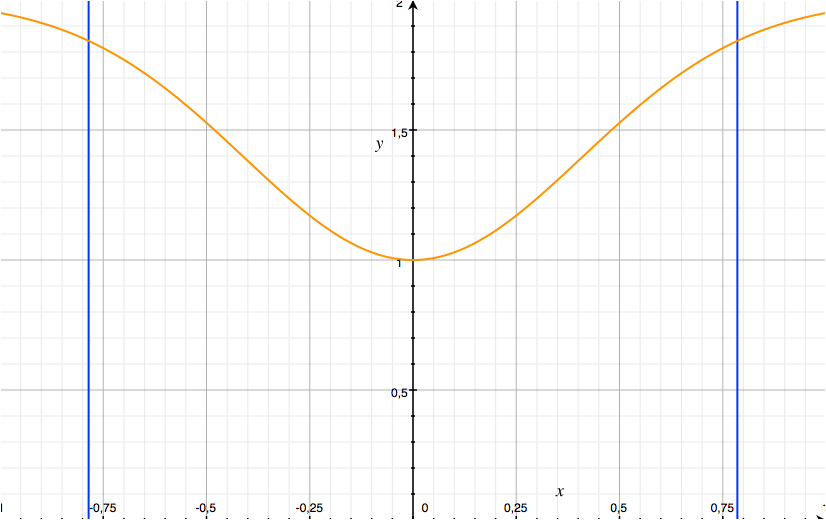
\includegraphics[width=\textwidth,height=\textheight,keepaspectratio]{assets/uss-function.jpg}
		\begin{tikzpicture}
		\datavisualization [
		scientific axes=clean,
		style sheet=strong colors,
		style sheet=vary dashing,
		all axes={grid},
		y axis={label=Verstärkung, ticks=few},
		x axis={label=Montagewinkel, ticks={step=15, tick unit=\degree}},
		visualize as smooth line/.list={func0,func25},
		func0={label in legend={text=Lenkwinkel $0\degree$}},
		func25={label in legend={text=Lenkwinkel $+25\degree$}},
		data/format=function
		]
		
		data [set=func0] {
			var x : interval [-45:45] samples 70;
			func y = 2 - e^(-3 * (\value x / 180 * pi)^2);
		}
		
		data [set=func25] {
			var x : interval [-45:45] samples 70;
			func y = 2 - e^(-3 * (\value x / 180 * pi - 25 * pi/180)^2);
		};
		\end{tikzpicture}
		
		\caption{Gewichtungsfunktion für verschiedene Lenkwinkel}
		\label{img-uss-function}
	\end{figure}

	
	

%%%%%%%%%%%%%%%%%%%%%%%%%%%%%%%%%%%%%%%%%%%%%%%%%%
\chapter{Kollisionserkennung}

	Mithilfe der Daten des Beschleunigungssensors werden Kollisionen erkannt und ein sofortiger Nothalt ausgelöst.
	\footnote{Dieses Feature befindet sich noch in Entwicklung.}
	
	Dabei wird darauf geachtet, dass die Ausschläge der Werte entsprechend hoch und kurzweilig sind, da auch bei starkem Abbremsen bereits starke aber anhaltende Beschleunigungen entstehen.
	

%%%%%%%%%%%%%%%%%%%%%%%%%%%%%%%%%%%%%%%%%%%%%%%%%%	
\chapter{Fahrbahnerkennung}

% TODO: Perspektivische Verzerrung erwähnen

\section{CPU vs. GPU}
Im Zusammenhang mit der Nutzung der OpenCV-Bibliothek sahen wir uns mit dem Problem, ob wir für die Bildverarbeitung die CPU oder die GPU verwenden, konfrontiert, da beides in OpenCV angeboten wird.

Standardmäßig wird der Code von OpenCV auf der CPU -- im Gegensatz zur GPU -- augeführt.
Während die OpenCV-CPU-Schnittstelle generell einfacher zu nutzen ist, bietet die GPU-Implementierung einen Performance-Vorteil, da GPUs für Matrixoperationen und die Arbeit auf 2D- und 3D-Bildern optimiert sind.
Diese Optimierung war trotz der echtzeitnahen Bildverarbeitung nicht zwingend notwendig.
Da das Modellauto allerdings mit einer aktuellen Grafikkarte -- der nVidia GeForce GTX 1050Ti -- ausgestattet ist, sahen wir in der GPU-Nutzung eine Möglichkeit, uns mit der Programmierung auf der GPU auseinanderzusetzen und Erfahrungen damit zu sammeln, weshalb wir uns für Programmcode entschieden haben, der weitestgehend auf der GPU ausgeführt wird.

Diese Entscheidung hatte wiederrum die Folge, dass der Code sich nicht auf PCs ohne nVidia-Grafikkarte ausführen lassen konnte, da die OpenCV-GPU-Implementierung auf der CUDA-Bibliothek basiert, die nur für nVidia-Grafikkarten nutzbar ist.
Dieses Manko nahmen wir in Kauf, und einige Gruppenmitglieder befassten sich mit der Konfiguration des nVidia-Treibers auf dem heimischen Rechner mit eigenen oder ausgeliehenen Grafikkarten, sodass auch der GPU-Code von zu Hause aus ausführbar war.

% NOTE: Erfahrungen a la "Blöd, zwischen GPU/CPU zu switchen?" -- "Doch ziemlich leichte Handhabung" -- "Wenig Codebeispiele" ?


\pagebreak

\section{Übersicht}

	\begin{figure}[ht]
		\centering
		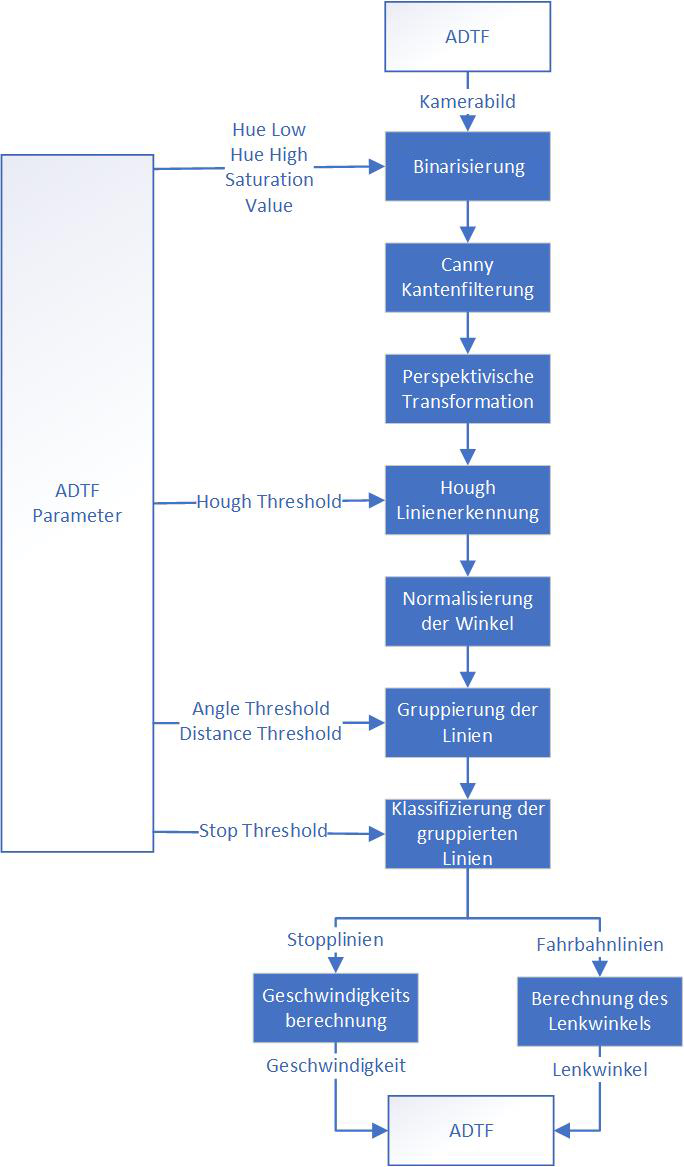
\includegraphics[width=250pt,keepaspectratio]{assets/bvaFlowchart.jpg}
		% NOTE: Tippfehler in "Binarisierung" entfernen. --hoe
		\caption{Übersicht der Bildverarbeitung}
		\label{img-bvaFlowchart}
	\end{figure}

\pagebreak

\section{Linienerkennung (Binarisierung)}	
	Die von einer Kamera (Realsense oder Basler) aufgenommene RGB-Bilder werden zunächst in das HSV-Farbmodell übertragen, um eine genauere Segmentierung anhand von Farben im Bild zu ermöglichen.
	Da die Fahrbahnmarkierung aktuell blau ist, wird der blaue Anteil von den anderen Farben im Bild getrennt. Die zugehörigen Parameter ($hue$, $saturation$ und $value$), die einen Unterraum des Farbraums bestimmen, können während der Laufzeit über die Eigenschaften des Filters in ADTF geändert werden, sodass auch Fahrbahnmarkierungen anderer Farben erkannt werden können.
	Das Ergebnis dieser Operation ist ein Binärbild es unterteilt die Pixel des HSV-Bilds in Pixel, die Teil des Unterraums sind (weiß) und solche, die nicht Teil des Unterraums sind (schwarz). Für die Bestimmung der Unterräume sowie die Binarisierung wird die OpenCV-Funktion \texttt{cv::inRange} genutzt.
	Damit potenzielle Löcher, die durch Rauschen entstehen können, geschlossen werden, wird ein Closing auf das Binärbild angewandt.

\section{Canny Edge Detection} %TODO vorher/nachher Bilder
	Um in dem Binärbild die Fahrbahnen als Linien erkennen zu können, wird ein Kantendetektionsverfahren -- der Canny Edge Detector, der bereits in OpenCV implementiert wurde -- verwendet (siehe auch \footnote{\url{https://docs.opencv.org/2.4/doc/tutorials/imgproc/imgtrans/canny\_detector/canny\_detector.html}}). Dieser erkennt in einem Grauwertbild mithilfe des Sobel-Operators Kanten, deren Stärke und Gewichtung pro Pixel aufgenommen wird. Um sicherzustellen, dass die Kanten nur einen Pixel breit sind, werden alle zu Kanten zugehörigen Pixel, die keine lokalen Maxima sind, aussortiert. Schließlich werden über zwei Schwellenwerte die Kantenkandidaten weiter gefiltert, sodass ein Binärbild entsteht. Ist die Kantenstärke eines Pixels größer als der obere Schwellenwert, wird der Pixel als Kante akzeptiert. Ist die Kantenstärke eines Pixels niedriger als der untere Schwellenwert, wird dieser Pixel als Kandidat verworfen. Über eine Hysterese werden die Pixel gefiltert, die zwischen beiden Schwellenwerten liegen, sodass "`Ausreißer"' vermieden werden. Dementsprechend nimmt die Funktion \texttt{cv::Canny}, bzw. das GPU-Pendant \texttt{cv::cuda::createCannyEdgeDetector} in Kombination mit der Funktion \texttt{detect}, die auf das Objekt angewandt wird, neben dem Bild folgende Parameter entgegen: \texttt{threshold1}, der die untere Grenze für die Aussortierung der Kandidaten bildet, \texttt{threshold2}, der die obere Grenze für die Aussortierung der Kandidaten bildet und \texttt{apertureSize}, die Größe des Sobel-Operators. Für das Verhältnis der Schwellenwerte zueinander wird das Verhältnis 2:1 bzw. 3:1 (\textit{upper:lower}) empfohlen.
	% NOTE: Das ist okay, aber ihr dürft davon ausgehen, dass der Leser weiß, wie der Canny Filter arbeitet. Ihr müsst die Parameter nicht erklären, es sei denn das war euch bei der Parameterwertsuche besonders wichtig. Konzentriert euch lieber auf die Beschreibung von dem, was ihr gemacht habt. :) --hoe
	
	Angewandt auf das binarisierte Bild der Straße hat der Canny-Algorithmus folgenden Effekt:
	
	% TODO Bilder!

\section{Hough Line Transformation}
	Nachdem die Kanten der Fahrbahnen nun gefiltert sind, können aus den Bilddaten die Fahrstreifen abstrahiert werden. Für die Positionsberechnung ist es notwendig, die Fahrbahnen nun in dem gefilterten Bild zu erkennen, und in geeigneter Weise zu mathematisch zu repräsentieren. \\
	OpenCV bringt die hierfür geeignete Hough Line Transformation mit. Diese transformiert das Bild in den Hough Raum. Über einen Threshhold Parameter kann hierbei die Empfindlichkeit des Filters eingestellt werden. Je niedriger, desto mehr Linien werden im Bild erkannt. Diesen Parameter kann im ADTF zur Laufzeit angepasst werden.\\
	Ebenfalls probierten wir zu Anfang noch die probabilistic Hough Transformation aus. Diese, ebenfalls von OpenCV mitgebrachte Funktion, hat die zusätzliche Eigenschaft, dass beispielsweise die gestrichelten Mittellinien nicht als eine einzelne Gerade erkannt werden, sondern jeder Strich der Mittellinie als einzelne Gerade. Da uns jedoch nur die Mittlline an sich interessiert, haben wir uns dazu entschieden, diese Transformation nicht zu verwenden. Dies reduziuert zudem die Menge der zu verarbeitenden Geraden.\\
	Die mit Hilfe der Hough Line Transformation erkannten Geraden werden in Polarkoordinaten dargestellt. Hierbei befindet sich der Ursprung oben links im Bild. Von diesem Punkt aus wird die Gerade mit einem Stützvektor mit dem Winkel $\theta$ und der Länge $r$ beschrieben.\\
	Aufgrund der Tatsache, dass das Bild so verzerrt wurde, dass wir die Straße aus einer senkrechten Obersicht betrachten, Entsprechen die Winkel der gefunden Geraden nun dem relativen Winkel der Fahrbahn zu unserem Model.
	
\section{Line-Clustering}
	% TODO Normalisierung der Linien erwähnen! (Grad)
	Durch die Hough Line Transformation werden tendenziell zu viele Linien gefunden. Um die Anzahl der Linien zu reduzieren, wird ein Clustering mithilfe der Funktion \texttt{cv::partition} verwendet, welches die Linien in Äquivalenzklassen unterteilt. Es wird eine Äquivalenzfunktion benutzt, die besagt, wann zwei Linien als äquivalent angesehen werden. Der Vergleich erfolgt anhand des Winkels des Normalenvektors der Linie und die Länge dieses Normalenvektors. Nach der Clusterung gibt es eine Zuordnung jeder Linie in eine Klasse. Alle Linien einer Klasse werden anschließend zu einer Linie zusammengefasst, indem Winkel und Abstand der Klasse zugehörigen Linien gemittelt werden.

\section{Klassifizierung}

\subsection{Haltelinien}

\section{Zentrierung in der Fahrspur}
	
	Bisher ist das Auto in der Lage der Fahrspur zu folgen.
	Allerdings besteht das Problem, dass es sich nicht in der Mitte der Spur zentriert.
	Dies führt dazu, dass es oft bereits auf den Linien fährt und teilweise sogar die andere Fahrspur mitbenutzt.
	Da es sich hierbei um unerwünschtes Verhalten handelt, thematisiert dieser Abschnitt unsere Herangehensweise.

\subsection{Theoretische Überlegungen}

	Angenommen es werden zwei Linien (linke und rechte Leitlinie) erkannt.
	Es wird nun jeweils der Abstand zur Seite ermittelt und dann gemittelt (Arithmetisches Mittel).
	Das Ergebnis ist ein Wert, der entweder links, rechts oder genau auf der Ideallinie des Fahrspur liegt.
	
	Es wird nun eine Funktion gesucht, die die Abweichung in eine Lenkanweisung umsetzt.
	Da dies schnell zu instabilem Verhalten führen kann, fällt eine lineare Funktion raus.
	Hier würde zu oft nachkorrigiert werden müssen.
	
	Unsere Wahl fiel daher auf eine modifizierte Sigmoid-Funktion:
	
		\[y=\frac{a_{max}}{1 + e^{-14\left( \frac{\left\|x\right\|}{x_{max}} - \frac{1}{2} \right)}} \cdot -\frac{x}{\left\|x\right\|}\]
	
	Hierbei steht $x$ für die aktuelle und $x_{max}$ für die maximale Abweichung von der Ideallinie.
	Der maximal anzusteuernde Lenkwinkel wird durch den Parameter $a_{max}$ angegeben.
	
	\paragraph{Veranschaulichung.} \autoref{img-spurzentrierung-function} zeigt die Funktion beispielhaft für eine maximale Abweichung von $x_{max} = 100mm$ und die damit einhergehende maximale Lenkwinkelreaktion von $a_{max} = 20\degree$.
	
	Je weiter sich das Auto von der Ideallinie entfernt, desto stärker wird der Lenkeinschlag und somit der Drang sich wieder zu zentrieren.
	
	Durch das exponentielle Verhalten ist sichergestellt, dass ein Aufschwingen unwahrscheinlich ist. Dies begründen wir dadurch, dass die Amplifikation um den Nullpunkt so gering ist, dass sie in der Praxis wie eine Totzone wirkt.
	
	\begin{figure}[ht]
		\centering
		
		\begin{tikzpicture}
		\datavisualization [
		scientific axes=clean,
		style sheet=strong colors,
		style sheet=vary dashing,
		all axes={grid}, scale=2,
		y axis={label=Lenkwinkel, ticks={few, tick unit=\degree}},
		x axis={label=Abweichung, ticks={step=50, tick unit=mm}},
		visualize as smooth line,
		data/format=function
		]
		
		data {
			var x : interval [-100:100] samples 20;
			func y = 20 / (1 + e^(-14 * (abs(\value x)/100 - 1/2))) * -\value x / abs(\value x);
		};
		\end{tikzpicture}
		
		\caption{Spurzentrierung mit $a_{max} = 20\degree$ und $x_{max} = 100mm$}
		\label{img-spurzentrierung-function}
	\end{figure}
	
	
	
	
\end{document}


